\section{Visualising the demographic spatio-temporal evolution}
\label{sec:method}
Figure~\ref{fig:overview} presents an overview of the processing steps of the
proposed method, illustrating how the nodes of the network are used to represent
the regions. The following sections elaborate this figure and explain the main
features of the interface we built to visualise and explore the evolution of
neighbourhoods on the basis of our proposed method.


\begin{figure}
    \centering 
    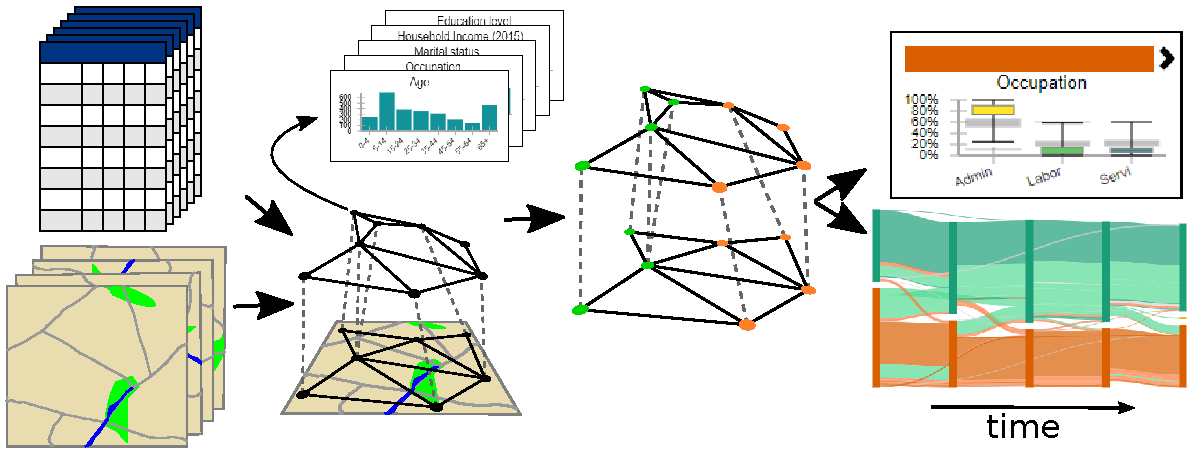
\includegraphics[width=0.975\linewidth]{overview.pdf}
    \caption{Overview of the proposed method. A network is generated combining the
        original census data, encoding the changing geographical information.
        The network is partitioned into an hierarchy~\citep{markus2017}. The
        characteristics and evolution of the clusters are then visually
        represented.
        \label{fig:overview}}
\end{figure}


\subsection{Census methodology and data representation}
\info{I removed any specifics of the experiments (CTs, which variables) from here because this section is theory}

Census data is disseminated in a tabulated form for aggregation areas: whole
country, state/province, metropolitan region, and so on. To allow for a more
meaningful comparison of the data, we aggregated related variables (e.g. White,
Black, Asian, Other) into what we called an \emph{aspect} (e.g. Race). The
aspects are represented using normalised histograms. This normalisation is
crucial for direct comparison. In essence, it is a generalisation of the
standard method of comparing percentages, since each aggregation area has a
different total population.

Each area of each census year is represented as a node, and edges are placed
between nodes if the corresponding regions share geographic borders in the same
year. Further, edges are placed between nodes if the corresponding regions
belong to sequential years and there is geographical overlap between them. This
approach leads to a single network representing the whole spatio-temporal space
of the data. Our objective then becomes to identify partitions of this network
such that the nodes of each partition are more similar between themselves than
to the other nodes. 


\subsection{Geographic content clustering}
Having tied the regions together into a network, we can now partition it to
identify similar sets of regions. We start by adopting a distance function
between the nodes, measuring the difference between the data of the regions.
This value is then associated with the edges, leading to a weighted dynamic
network. Every node has a collection of histograms, each representing the
distribution of certain aspect in the population.

Let $\G=(\V,\E)$ be a network, where
$\V=\{\vertice_1,\vertice_2,\dots,\vertice_n\}$ is the set of nodes and
$\E=\{(\vertice_i,\vertice_j), i\not=j\text{ and }i,j \in [1,n]\}$ is the set of
edges. A function $\Hist$ associates each node to a set of $K$ histograms. We
define the distance $\D$ between two nodes $\vertice_i$ and $\vertice_j$ as:

\begin{equation}
    \D(\vertice_i,\vertice_j)=\sum_{k \in [1,K]}{\weight_k\, d(\Hist_k(\vertice_i),\Hist_k(\vertice_j))}
    \label{eq:dist}
\end{equation}

\noindent where $d$ is a distance metric between histograms and $\weight$ is a
sequence of non-negative weights associated with each aspect,
$\sum_{k\in[1,K]}{\weight_k}=1$. While any histogram metric can be used, we
adopted a euclidean distance between the vectors, because it led to reasonable
results with reduced computational cost. Therefore the distance between two
nodes is defined as the weighted average distance between its associated
histograms, where the weights can be adjusted by the user.

Once the distances are associated to the edges, we use watershed
cuts~\citep{Cousty2009} to create an initial clustering, which is then refined
into a hierarchy using the Sorted Maximal Matching (SMM)~\citep{markus2017} with
median linkage. The initial watershed step is performed to create an initial
clustering and reduce the running time of the SMM. We introduced one new
parameter to this method: a maximum distance threshold for the merges, to avoid
the early merging of outliers. We refer the reader to the original
paper~\citep{markus2017} for more details, including a complete performance
evaluation using several metrics.


Each resulting cluster is contiguous in the network. This means that two
similar, but non-contiguous, sets of areas will be classified into two different
clusters, which can be counter-intuitive. To overcome this issue, we
\emph{augment} the network with two new edges per node from a nearest neighbours
graph~\citep{scikit-learn} using only the distances between the histograms.
These edges connect nodes with similar content, if they are not already
connected, providing a path for the algorithm to group similar nodes.


\subsection{Cluster characterisation and variable relevance}
\label{sec:relevance}
A crucial step in understanding neighbourhood change is to characterise the
evolving clusters.  The composition of each cluster is represented here by
simple statistical measures, considering each aspect separately. We compute the
minimum, maximum, median, 25\%, and 75\% quantiles for each variable of each
aspect for all clusters in the hierarchy. While interpreting these values is
more complex than interpreting just the average, they provide far more
information about the underlying distribution.


We also use these statistical measurements to discover what characterises each
cluster, that is, what makes it different from the others.  We define the
\emph{relevance} of a variable of an aspect based on the distance between the
interquantile ranges (IQR) of the clusters in the same hierarchical level. If
the IQRs overlap for all clusters, that variable is not relevant to the
characterisation of the cluster, but if the IQRs are distant, it means that this
specific range of values is something that only occurs in this cluster.
Examining IQRs therefore provides users a straightforward visual method for
determining what variables most clearly define a given cluster.


\subsection{Clusters and trajectories}
While the partition of the data into different clusters helps the user to
understand what groups exist and where they are, we are also interested in the
evolution of these groups. To examine this process of evolution directly, we
introduce the concept of \emph{trajectories}. Trajectories are composed by
regions classified into the same sequence of clusters over the considered
period. This enables direct access to regions that evolved in the same manner.
While individual census tracts remain interesting, these trajectories are the
main unit of exploration in this work.


\subsection{User interface}
\label{sec:ui}
To validate and explore the results of our methodology, we built a user
interface, illustrated in Figure~\ref{fig:ui}, considering census tract (CT)
level data from the Chicago region between 1970 and 2010. This region is known
for its entrenched racial divide and the emergence of a \emph{'young urban'}
population with a higher education level~\citep{Delmelle2016,Delmelle2017}. More
details are presented in Section~\ref{sec:study}.


\begin{figure*}
    \centering 
    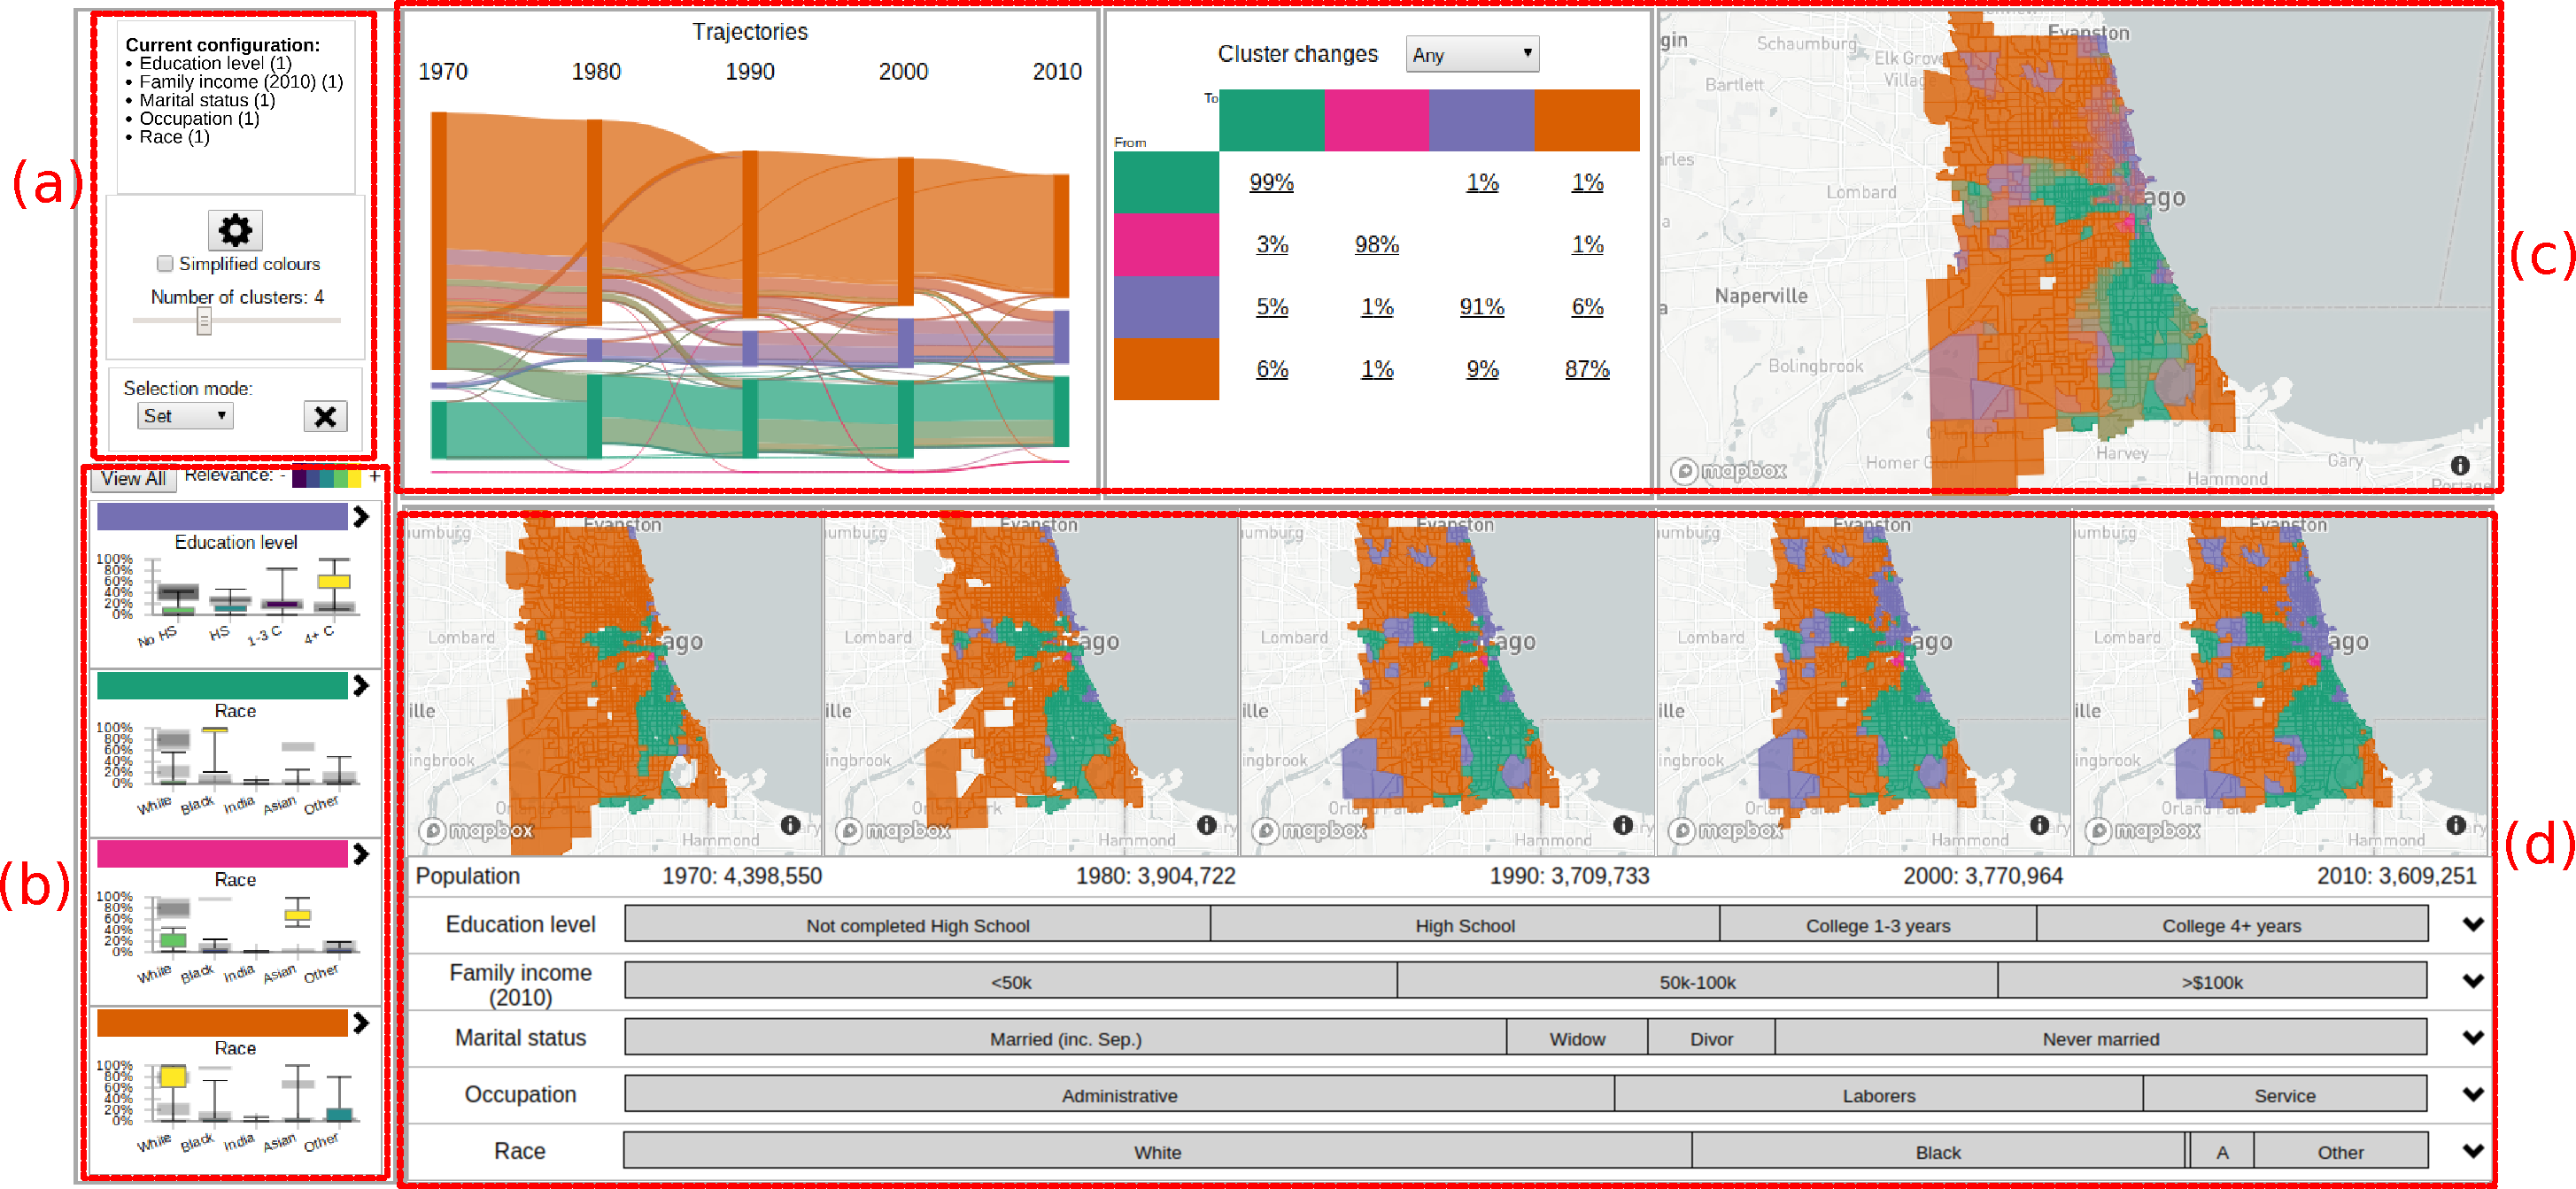
\includegraphics[width=0.975\linewidth]{ui.pdf}
    \caption{Initial interface of our method showing the demographic evolution of Chicago. 
        \textbf{(a)}: Configuration panel with the current clustering parameters and controls.
        \textbf{(b)}: Cluster overview illustrating the most relevant aspect for each cluster. 
        \textbf{(c)}: Trajectories overview and the general evolution of the population, geographical information, and how it changed. 
        \textbf{(d)}: Details of the selected trajectories, including precise geographic locations, population numbers, and the composition of the aspects.\label{fig:ui}}
\end{figure*}


As illustrated by Figure~\ref{fig:ui}, our proposed interface heavily relies on
colour to express cluster-related information. We adopted this convention
because colours can be used in all our visual tools in a coherent manner.
However, there is a limit on the number of distinct colours that can be used. We
limited the number of clusters to eight because this was the largest number of
colours that we could reliably and accessibly use, derived from the 8-class
Dark2 set from ColorBrewer~\citep{ColorBrewer}. 


The configuration panel, on top left in Figure~\ref{fig:ui}, displays which
aspects were used and their weights (following Equation~\ref{eq:dist}). It also
includes other configuration options that can be altered without re-processing
the data, such as the number of clusters and the colour option. The gear button
allows access to the other configuration options that do require further
processing, such as changing location, aspects, and weights. 


The cluster overview panel, on the bottom left in Figure~\ref{fig:ui}, displays
a brief summary of each cluster, based on the distance between the IQRs, as
detailed in Section~\ref{sec:relevance}. The \emph{View all} button opens a new
panel where all aspects are included, while the chevron at the side lets the
user expand each cluster separately. 

We adopted an \emph{enhanced} version of the traditional boxplot, which includes
the IQRs for the other clusters, in slightly larger and faded black rectangles.
We also colour the current IQR according to its relevance.  For instance, the
boxplot that summarises the purple cluster illustrated in Figure~\ref{fig:ui},
detailed on Figure~\ref{fig:boxplot}, illustrates that this cluster is best
defined by the proportion of the population with four or more years of college.
The user can quickly see that this is relevant because the corresponding IQR is
coloured with the highest relevance present in the legend. It is also clear
that, while this cluster includes CTs that have between 10\% to 90\% of people
in this variable, approximately, half of them have about 60\% of the population
with four or more years of college. Since all the other IQRs are well separated,
this is a defining characteristic of this cluster. Conversely, the proportion of
the population with one to three years of college is not relevant, as indicated
by black fill in the rectangle representing the IQR of this cluster, in
overlapping position with the rectangles of the other clusters. By clicking on
the coloured bar above the boxplot, the user can select all trajectories that
contain this cluster at any point in time.

\begin{figure}
    \centering 
    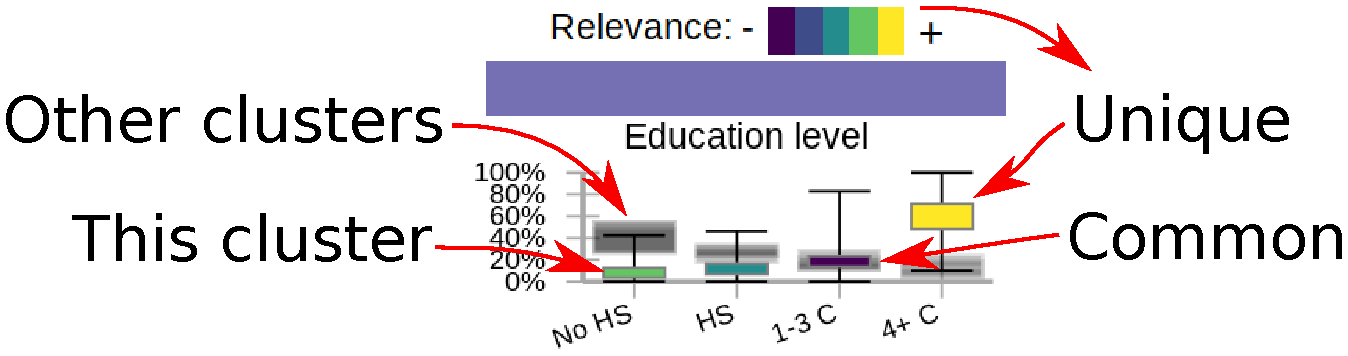
\includegraphics[width=0.45\linewidth]{boxplot.pdf}
    \caption{Enhanced boxplot of the clusters' characteristics allows a quick
    comparison to the other clusters.\label{fig:boxplot}}
\end{figure}


The trajectories overview aims to convey basic information about the
trajectories, where they are, and what changes are involved. This is done using
three sub panels. The first, on the left, contains a Sankey diagram illustrating
the evolution of the clusters over time. The widths are proportional to the
population involved. In our example in Figure~\ref{fig:ui}, the orange and green
clusters contain most of the population and are fairly stable over time. The
pink cluster is small and mostly stable. The purple cluster is increasing,
mostly by incorporating areas that were previously orange. Since the purple
group corresponds to the emergent 'young urban' group, this corroborates the
findings of Delmelle~\citep{Delmelle2016,Delmelle2017}, showing that our
network-based method can recover results from the traditional data processing
approach.

In the next panel, illustrated in the top middle of Figure~\ref{fig:ui}, is a
transition matrix between the clusters. It indicates a rounded percentage of the
population whose area changed between each pair of clusters. This kind of table
can be found in the related literature~\citep{Delmelle2016}, so it is familiar
to the advanced users. It not only informs the proportional changes, but allows
the selection of the corresponding trajectories for further analysis.

The panel in the top right of Figure~\ref{fig:ui} is a map of the region under
analysis, summarising the geographical evolution of the clusters over time.  The
colours are derived from the clusters involved in each trajectory, which are
consistent across the linked views. 

The bottom part of the interface contains the details for the selected
trajectories, or for the whole city if nothing is selected, as illustrated in
Figure~\ref{fig:ui}. This panel contains two main regions: the small multiple
maps, depicting the clusters at each year, and the stacked bar plots that
summarise the overall composition of these regions. In this example, the maps
show the transition from orange to green and purple in several regions over
time. Clicking on a region in these maps will bring up a new panel with the
original census data of this specific region. The actual population numbers are
below the maps.

Each aspect is represented by a stacked bar plot, where the width of each
rectangle corresponds to the average percentage of that variable over the
considered period. In this case, about half of the people in Chicago in the
considered period are married, and the percentage that are Widowers or Divorced
is roughly similar. About half of the population work in Administrative jobs, a
third never completed high-school, approximately half have gross family income
below 50,000USD per year. The vast majority identify as white. Placing the mouse
over one of the bars will open a small panel with the temporal evolution of that
specific variable, and clicking on the chevron on the right side expands the
corresponding aspect, showing details of the temporal evolution of each variable
and also the corresponding IQRs for the whole city.